\documentclass[a4paper]{article}
\usepackage[spanish]{babel}  %babel es el paquete de idiomas y antes de eso va el o los idiomas que se reuqieren emplear
\usepackage[colorlinks=true, citecolor=blue, final]{hyperref}
\usepackage{url} % UTILIZA EL PAQUETE PARA QUE APAREZCA EL URL AUNQUE AUN NOSE SI DEBO ACTIVARLO TAMBIEN EN REFERENCIAS
\hypersetup{
    colorlinks=true,
    linkcolor=blue,
    filecolor=blue,      
    urlcolor=blue,
}
\usepackage{graphicx}
\usepackage[sort&compress, numbers]{natbib}
\usepackage{xcolor}
\usepackage{listings}
\usepackage{ragged2e}
\definecolor{codegreen}{rgb}{0,0.6,0}
\definecolor{codegray}{rgb}{0.5,0.5,0.5}
\definecolor{codepurple}{rgb}{0.58,1,0.82}
\definecolor{backcolour}{rgb}{1,1,0.97}
\lstdefinestyle{mystyle}{
    backgroundcolor=\color{backcolour},   
    commentstyle=\color{codegreen},
    keywordstyle=\color{magenta},
    numberstyle=\tiny\color{codegray},
    stringstyle=\color{codepurple},
    basicstyle=\ttfamily\footnotesize,
    breakatwhitespace=false,         
    breaklines=true,                 
    captionpos=b,                    
    keepspaces=true,                 
    numbers=left,                    
    numbersep=5pt,                  
    showspaces=false,                
    showstringspaces=false,
    showtabs=false,                  
    tabsize=2
}
\lstset{style=mystyle}


\begin{document}  %se utiliza para comenzar lo señalado en el parentesis
\begin{center} %begin para comenzar  agregamos centrar para poner en medio
\large \bf Práctica Nº 3   %\large aumenta ligeramente el texto posterior o alarga 
\\ %\\ Indica brincar espacio. \bf indicara subrayar en negritas las letras despues antes de el termino checar que este en minusculas aveces no entra no se porque pasa un espacio antes y despues de agregar
Teoría de colas
\end{center} %end terminacion de lo señalado en corchetes en este caso el centrado
\textbf{Nombre:}   %\Textbf marca en negritas la frase entre los corchetes
José Adrián García Fuentes
\hfill  %hfill genera un espacio horizontal para expandirse a lo largo del documento
\textbf{Profesor:}   %para que entre el textbf checar que este todo en minusculas
Satu Elisa Schaeffer \hfill
\\
\textbf{Fecha:} 02/Marzo/2021        %\today agrega la fecha en formato de mes dia, año en ingles agregar un usepackage al principio entre llaves el idioma a emplear y entre corchetes babel que es el paquete de idiomas
\\
\hrule    %hrule agrega una linea horizontal en el documento
\medskip
   %bigskip hace espacio grande entre parrafos medskyp tamaño medio y small skyp uno pequeño  si solo pasas espacios no se despega de una linea y marca error
 \section{Introducción}
\justify La teoría de colas es un área de las matemáticas que estudia el comportamiento de líneas de espera. Los trabajos que están esperando ejecución en un cluster esencialmente forman una línea de espera \cite{p3}.
\section{Objetivo}  %\section da enfasis a empezar una nueva seccion o tema
\begin{itemize}   %begin comenzar itemize es una viñeta se marca como item no es necesario agregar espacio despues de cada item
    \item Examinar cómo las diferencias en los tiempos de ejecución de los diferentes ordenamientos cambian cuando se varía el número de núcleos asignados al cluster, utilizando como datos de entrada un vector que contiene primos grandes, descargados de \url{https://primes.utm.edu/lists/small/millions/} y no-primos (creados a partir de ellos) con por lo menos nueve dígitos, aplicando pruebas estadísticas adecuadas y visualización científica clara e informativa \cite{p3}. 

\end{itemize}

%\\ Indica brincar espacio.
\section{Metodología}
\justify
La metodología empleada se realizó a través de RStudio\cite{RStudio} llevando a cabo los pasos señalados en la \textit{Práctica 3: teoría de colas} \cite{p3}, se examinaron las diferencias en tiempos de ejecución de los diferentes ordenamientos cuando se varia el numero de nucleos asignados al cluster, utilizando como datos de entrada del vector utilizando primos grandes, el código completo de la metodología empleada se encuentra en el repositorio \cite{gitadrian} del autor.


\section{Resultados}
\justify
Se obtuvo el código secuencia para determinar si un número es primo o no primo, a partir de este experimento se determino el tiempo que tardaba en detectar si era primo o no primo. A continuación se muestra parte del código del experimento \cite{gitadrian} en el cual se señala el número de repeticiones y parte de la función dada solicitando números de manera pseudoaleatoria que determinaran la posición final de nuestro punto, dicho código fue modificado de el código del docente \cite{p3gitdr}. 

 \begin{table}[h!]
     \centering
          \caption{Registro de tiempos}
     \begin{tabular}{c|c|c|c}
           min & max & promedio & media  \\
           0.20 & 0.72 & 0.50 & 0.48  \\
           0.1 & 0.21 & 0.19 & 0.16  \\
           0.03 & 0.20 & 0.10 & 0.12 \\
     \end{tabular}
     \label{tab:my_label}
 \end{table}
 
\begin{lstlisting}
library(parallel)
detectCores(-1)
primo <- function(n) {
  if (n < 4) {
    return(TRUE)
  }
  if (n %% 2 == 0) {
    return(FALSE)
  }
  for (i in seq(3, max(3, ceiling(sqrt(n))), 2)) {
    if (n %% i == 0) {
      return(FALSE)
    }
  }
  return(TRUE)
  for (noprimo in (valoresprimos[1] + 1):(valoresprimos[2]-1))
  {print(noprimo)}
}
\end{lstlisting}
\justify A continuación en la Fig \ref{practica3.png} se muestra un diagrama caja bigote de el tiempo de interacción al correr el experimento. 
\begin{figure}[h]
    \centering
     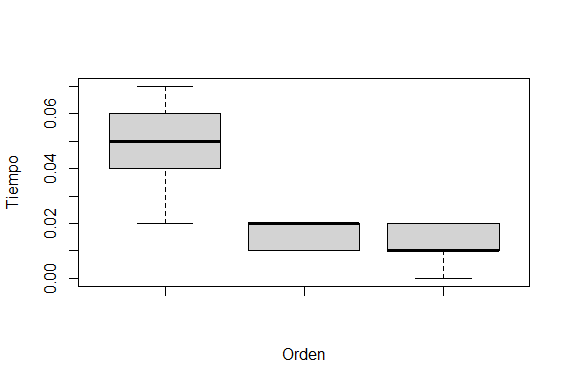
\includegraphics[width=60mm]{practica3.png}
    \caption\\Diagrama caja bigote{\label{practica3.png}
    \label{practica3.png}}
\end{figure}
 
\section{Reto 1}
 Modificar la tarea por realizar a que se encuentren todos los divisores del número (es decir, todos los enteros mayores a uno y menores al número mismo que lo dividen exactamente y examinar si las conclusiones cambian.
 
\begin{lstlisting}
divisor<- function (n) {
       div<-numeric()
       for (i in 1:ceiling(sqrt(n))){
           if ((n %% i)= 0){
              div<-c(div,i)
              div<-c(div,n/i)
              }
        }
        return(sort(unique(div)))
    }
\end{lstlisting}

 \section{Reto 2}
 Modificar el primer reto a que encuentre solamente los factores y sus multiplicidades, es decir, que encuentre para n aquellos números primos $1 < p < n$ y sus potencias para que el producto de los factores con esas potencias de n. Nuevamente hay que examinar si este cambio afectó las conclusiones del experimento de la tarea.
 
 \begin{lstlisting}
fact_primos<-function(n){
    div<-numeric()
    if(n==1){
        return(1)
    }
    while(n%%2 == 0){
    div<-c(div,2)
    n = n/2
    }
    for(i in seq(3, max(3, ceiling(sqrt(n))), 2)){
        while(n%%i==0){
            div<-c(div,i)
            n=n/i
        }
    }
    if(n>2){
        div<-c(div,n)
        }
    return(table(div))
}
 \end{lstlisting}

\section{Conclusión}
\justify En conclusión el tiempo en que tarda un experimento en correr una secuencia variando el numero de nucleos de un cpu puede ser mas corto de pendiendo de que tan largo sea el experimento

\clearpage
\bibliography{practica3} %\bibliography dentro de los corchetes aparece el comando seccion de referencias  sin embargo para que aparezca tiene que aparecer la seccion \bibliographystyle para dar un estilo del tipo de letra o tipo de acomodo que llevara 
\bibliographystyle{ieeetr}   %\da un estilo de acomodo dependiendo del comando dentro d corchetes
\end{document} %indica finalizacion de lo señalado en el parentesis en este caso el documento

